
%% bare_conf.tex
%% V1.4a
%% 2014/09/17
%% by Michael Shell
%% See:
%% http://www.michaelshell.org/
%% for current contact information.
%%
%% This is a skeleton file demonstrating the use of IEEEtran.cls
%% (requires IEEEtran.cls version 1.8a or later) with an IEEE
%% conference paper.
%%
%% Support sites:
%% http://www.michaelshell.org/tex/ieeetran/
%% http://www.ctan.org/tex-archive/macros/latex/contrib/IEEEtran/
%% and
%% http://www.ieee.org/

%%*************************************************************************
%% Legal Notice:
%% This code is offered as-is without any warranty either expressed or
%% implied; without even the implied warranty of MERCHANTABILITY or
%% FITNESS FOR A PARTICULAR PURPOSE! 
%% User assumes all risk.
%% In no event shall IEEE or any contributor to this code be liable for
%% any damages or losses, including, but not limited to, incidental,
%% consequential, or any other damages, resulting from the use or misuse
%% of any information contained here.
%%
%% All comments are the opinions of their respective authors and are not
%% necessarily endorsed by the IEEE.
%%
%% This work is distributed under the LaTeX Project Public License (LPPL)
%% ( http://www.latex-project.org/ ) version 1.3, and may be freely used,
%% distributed and modified. A copy of the LPPL, version 1.3, is included
%% in the base LaTeX documentation of all distributions of LaTeX released
%% 2003/12/01 or later.
%% Retain all contribution notices and credits.
%% ** Modified files should be clearly indicated as such, including  **
%% ** renaming them and changing author support contact information. **
%%
%% File list of work: IEEEtran.cls, IEEEtran_HOWTO.pdf, bare_adv.tex,
%%                    bare_conf.tex, bare_jrnl.tex, bare_conf_compsoc.tex,
%%                    bare_jrnl_compsoc.tex, bare_jrnl_transmag.tex
%%*************************************************************************


% *** Authors should verify (and, if needed, correct) their LaTeX system  ***
% *** with the testflow diagnostic prior to trusting their LaTeX platform ***
% *** with production work. IEEE's font choices and paper sizes can       ***
% *** trigger bugs that do not appear when using other class files.       ***                          ***
% The testflow support page is at:
% http://www.michaelshell.org/tex/testflow/



\documentclass[conference]{IEEEtran}
% Some Computer Society conferences also require the compsoc mode option,
% but others use the standard conference format.
%
% If IEEEtran.cls has not been installed into the LaTeX system files,
% manually specify the path to it like:
% \documentclass[conference]{../sty/IEEEtran}

\usepackage{amsmath}

% Some very useful LaTeX packages include:
% (uncomment the ones you want to load)
% ---
% PACOTES
% ---
\usepackage[english,american,brazil]{babel}		% Idioma do documento
\usepackage{color}			% Controle das cores
\usepackage[T1]{fontenc}		% Selecao de codigos de fonte.
\usepackage{graphicx}			% Inclusão de gráficos
\usepackage[utf8]{inputenc}		% Codificacao do documento (conversão automática dos acentos)
\usepackage[noadjust]{cite}
\usepackage{txfonts}			% Fontes virtuais
\usepackage{listings}
\usepackage{adjustbox}
\usepackage{tabularx}
\usepackage{multirow}
\usepackage{multicol}
\usepackage{colortbl}
\usepackage{caption}
\usepackage{microtype} 			% para melhorias de justificação
\usepackage{lipsum}
\usepackage{datetime}
\usepackage{float} %use the “float” package and then the [h] option for your figure.
\usepackage{hyperref}
\usepackage{pgf}
\usepackage{tikz}
\usetikzlibrary{arrows,shapes,automata,positioning}


\usepackage{filecontents}
% correct bad hyphenation here
\hyphenation{op-tical net-works semi-conduc-tor}

\begin{document}
%
% paper title
% Titles are generally capitalized except for words such as a, an, and, as,
% at, but, by, for, in, nor, of, on, or, the, to and up, which are usually
% not capitalized unless they are the first or last word of the title.
% Linebreaks \\ can be used within to get better formatting as desired.
% Do not put math or special symbols in the title.
\title{Estudo e modelagem para o sistema de controle supervisório em veículos autônomos terrestres}

% author names and affiliations
% use a multiple column layout for up to three different
% affiliations
\author{
	\IEEEauthorblockN{Carlos F. de P. Perché}
	\IEEEauthorblockA{Faculdade de Engenharia Mecânica - {UNICAMP}\\
	Campinas, SP, Brasil 13083--000\\
	Email: cfpperche@gmail.com}
}

% make the title area
\maketitle

% As a general rule, do not put math, special symbols or citations
% in the abstract
\begin{abstract}

Obter total controle das atividades em veículos autônomos terrestres continua a ser uma questão em aberto devido a crescente complexidade inerente aos demais sistemas que compõe este tipo de aplicação. Para isso, avançadas estratégias de controle supervisório devem ser desenvolvidas para que se possa fazer o uso da capacidade total destes sistemas. A principal função do controle supervisório é monitorar e coordenar as atividades dos componentes de tal forma que o comportamento geral do veículo cumpra determinados requisitos.

Neste artigo, é apresentado o estudo e a modelagem de uma arquitetura para o componente responsável pela supervisão operacional em veículos autônomos terrestres e a proposta preliminar para sua implementação com base em abordagens formais dos sistemas de controle para eventos discretos. Sob a arquitetura proposta, o controle supervisório é obtido através de uma estrutura uniforme de transições "genéricas" modeladas por máquinas de estados finitos para os sistemas presentes no veículo. Esta estrutura tem o objetivo de fornecer um "comportamento" determinístico para o sistema como um todo, facilitando o cumprimento dos requisitos necessários para a execução das operações executadas. 

O trabalho propõe uma solução que possibilite a coordenação dos componentes que compõem veículos autônomos terrestres tanto a nível comportamental quanto operacional, realizando o monitoramento das tarefas e a garantia  da integridade do veículo.

%A aplicabilidade do quadro proposta é ilustrada através de um cenário simples de terreno aberto.
%The applicability of the proposed framework is illustrated by using a simple scenario of open terrain.

%Dentro deste quadro de supervisão de controle do veículo é implementado em ambos os níveis comportamentais e operacionais para a coordenação módulo, comutação comportamento do veículo, monitoramento e supervisão tarefa operação do sistema.
%Within this framework supervisory control of the vehicle is implemented at both behavioral and operational levels for module coordination, vehicle behavior switching, task monitoring and system operation supervision.


%É discutido implicação da adoção desta estrutura de transição de estado sobre a possível síntese formal de controle de supervisão.
%Implication of adopting this state-transition structure on possible formal synthesis of supervisory control is discussed.

%Esta estrutura representa um subconjunto do comportamento de cada componente que é reconhecida pelo controlador de supervisão, o qual é concebido com o objectivo de atingir um determinado comportamento do veículo.
%This structure represents a subset of the behavior of each component that is recognized by the supervisory controller, which is designed with the objective of achieving certain behavior of the vehicle.


%Sob essa arquitetura, o controle do veículo de supervisão é conseguido através uniformemente adotar uma estrutura de transição de estado "genérico" para cada componente no veículo.
%Under this architecture, supervisory control of the vehicle is achieved by uniformly adopting a "generic" state-transition structure for each component in the vehicle.


%Neste artigo, apresentamos o projeto de uma arquitetura de controle de supervisão e sua implementação preliminar de um veículo de terra capaz de operação autônoma em terreno aberto.
%In this article, we present the design of a supervisory control architecture and its preliminary implementation for a land vehicle capable of autonomous operation in open terrain.

%A estrutura é apresentada neste artigo para o controle de supervisão reforçada de tais sistemas com base em abordagens formais de sistemas de eventos discretos e teoria de controle de supervisão.
%A framework is presented in this paper for the enhanced supervisory control of such systems based on formal approaches of discrete event systems and supervisory control theory. 


%A principal função de um controlador de supervisão é monitorar e coordenar as atividades dos componentes de tal forma que o comportamento geral do veículo cumpra determinados requisitos.
%The main function of a supervisory controller is to monitor and coordinate the activities of the components such that overall behavior of the vehicle meets certain requirements.


%Resolver este problema exige não apenas componentes sofisticados para a actuação, a detecção e comunicação, mas também estratégias de controle de supervisão avançados que podem fazer uso da capacidade total dos componentes.
%Solving this problem requires not only sophisticated components for actuation, sensing, and communication, but also advanced supervisory control strategies that can make use of the full capability of the components. 


%Alcançar operação autônoma por um veículo não tripulado em terreno aberto continua a ser um problema desafiador no desenvolvimento de veículos terrestres.
%O controle de supervisão de veículos terrestres não tripulados, devido à sua crescente complexidade inerente tornou-se um componente muito importante.

%Achieving autonomous operation by an unmanned vehicle in open terrain remains a challenging problem in the development of land vehicles. 
%The supervisory control of unmanned ground vehicles due to their inherent growing complexity has become a very important component.
\end{abstract}

\begin{IEEEkeywords}
unmaned land vehicle, supervisory control, finite state machine, critical real-time system, discreve event system.
\end{IEEEkeywords}


\IEEEpeerreviewmaketitle
% -------------------- NEW SECTION -------------------- 
% -------------------- NEW SECTION -------------------- 
% -------------------- NEW SECTION -------------------- 
\section{Introduction}\label{sec:introduction}
Veículos autônomos terrestres precisam ser equipados com uma variedade de componentes para o processamento de dados, comunicação, atuação, sensoriamento, etc. A complexidade destes componentes tem crescido e cada vez mais eles desempenham suas funções de forma independente. Uma vez que estejam devidamente integrados e coordenados, eles tornam capaz a navegação autônoma guiando o veículo com a mínima intervenção humana \cite{autonomous_Hebert:1997:IUG:523961} \cite{autonomous_doi:10.1117/12.391642}.

Obter comportamento autônomo em um veículo terrestre ainda continua a ser uma questão desafiadora, principalmente devido a complexidade que o ambiente de operação apresenta. A superfície terrestre possui uma grande variedade de características que tornam até a navegação manual uma tarefa difícil. Um veículo que possui bom desempenho de operação em terrenos montanhosos pode não possuir a mesma eficiência em ambientes tropicais. Outras condições ambientais, como as questões climáticas ou temporais, também interferem significativamente na performance dos veículos terrestres \cite{supervisory_Donmez:2010:MSE:2377576.2377580}. 

A solução para tais problemas requerem além da utilização de sofisticados componentes para processamento, comunicação, atuação e sensoriamento, mas também uma boa estratégia de controle supervisório capaz de possibilitar que os componentes possam utilizar o máximo de sua capacidade, sem que haja significativa degradação na performance do sistema \cite{supervisory_Cummings_1a}. A principal função de um sistema supervisório é o monitoramento e coordenação das atividades em execução nos componentes, para que de forma geral, o veículo cumpra os objetivos determinados, que podem variar desde mover de um local para outro no menor tempo possível, ou simplesmente seguir outro veículo a sua frente à uma distância "segura". 

Além disso, é preciso levar em conta que este tipo de aplicação é caracterizado como um sistema crítico de tempo real \cite{rtos_safety_mission_4062424} \cite{rtos_analysis_336046}, onde alternativas para garantir que determinadas tarefas sejam cumpridas em um período de tempo especificado, caso contrário, falhas graves ocorreram tornando o projeto inviável \cite{rtos_nasa_monitors} \cite{rtos_choosing_barr2003choosing}.

Neste trabalho é apresentado a proposta da arquitetura de controle supervisório para o veículo VILMA \cite{lma_vilma_website} e seu processo de desenvolvimento, visando a obtenção de operações autônomas em ambientes terrestres, levando em consideração os requisitos necessários para os sistemas críticos de tempo real. Sob a arquitetura proposta, é adotada uma interface uniforme que deve ser incorporada aos sistemas que compõem o veículo além de uma plataforma que possibilite o desenvolvimento do projeto. A interface adotada representa um conjunto comportamental, onde cada componente presente na arquitetura do veículo possa ter suas tarefas gerenciadas pelo supervisório, possibilitando que as operações realizadas pelo veículo tenham caráter determinísticos.

O restante desta dissertação está organizada da seguinte forma. A Seção \ref{sec:architec_concepts} descreve os conceitos e a metodologia utilizada para a arquitetura de supervisão e lista os objetivos e requisitos pretendidos. A Seção \ref{sec:proposed_architec} descreve o comportamento geral do veículo autônomo VILMA, apresenta os módulos e componentes presentes na arquitetura do veículo, descreve a estrutura de transições de estados para as tarefas a serem executadas em um componente onde as estrategias de controle supervisório atuam de acordo com o comportamento esperado e aborda uma possível metodologia para uma síntese formal de controle para a arquitetura proposta. A Seção \ref{sec:architec_components} apresenta os elementos de software utilizados para a plataforma de desenvolvimento da arquitetura. A Seção \ref{sec:implementation} traz uma descrição preliminar sobre a implementação da arquitetura de controle supervisório. Por fim, a Seção \ref{sec:conclusion} concluí este trabalho.

% -------------------- NEW SECTION -------------------- 
% -------------------- NEW SECTION -------------------- 
% -------------------- NEW SECTION -------------------- 
\section{Architecture Concepts}\label{sec:architec_concepts}

Um veículo autônomo terrestre (VAT) é composto por diversos sistemas que possuem funções específicas, como percepção do ambiente local, controle da navegação, localização global, etc., todos operando em paralelo. Tipicamente um VAT possui o modo de operação manual, forma convencional com que os veículos são operados, e modo autônomo, que possui um completo controle computacional que determina sua "inteligência".

O avanço das pesquisas envolvendo VATs tem resultado no aumento do nível de complexidade e volume de dados em seus sensores e sistemas específicos, gerando a necessidade de distribuir o processamento das informações em vários "computadores embarcados" que se comunicam de forma sincronizada. Assim, uma adequada supervisão dos módulos é essencial para um projeto modular com características determinísticas. Este gerenciamento deve realizar o controle das atividades de acordo com o as necessidades de cada tarefa e garantir o comportamento do veículo baseado em regras que priorizem as operações seguras.

Além disso, o desenvolvimento de um VAT necessita ser adaptável para todos os requisitos funcionais nos diversos cenários de operação em que o veículo possa realizar suas tarefas. Neste contexto, o sistema controle supervisório precisa verificar a integridade dos demais módulos que realizam, por exemplo, a leitura dos sensores, o controle de velocidade ou o sistema de posicionamento. Ou seja, verificar constantemente a presença e o comportamento destes sistemas.

Técnicas formais como maquinas de estado finitas (FSM, do inglês \textit{finit state machine}) para modelar o comportamento de sistemas determinísticos e realizar sua supervisão tem sido utilizadas em diversas áreas que incluem comunicação em rede, sistemas de controle trafego, linhas de montagem, e assim por diante \cite{event_comparative_study} \cite{event_des_line_945770}. 

Esta mesma técnica tem sido apresentada por pesquisadores em trabalhos relacionados, como aplicações robóticas e sistemas de veículos autônomos. \cite{event_supervisory_soccer_994642} utiliza um conjunto de FSMs para descrever o comportamento colaborativo de robôs para partidas de futebol. \cite{event_hybrid_automata_827799} modela um robô autônomo utilizando um sistema hibrido de autômatos onde a alteração de seu comportamento é modelada por FSMs contendo estados discretos que correspondem a comportamentos distintos através de um modelo contínuo. \cite{event_modular_navigation} apresenta uma aplicação onde seu comportamento é baseado em modelagem por maquinas de estados para um sistema de navegação modular em um veículo que opera sob tuneis.

Os trabalhos descritos tem como objetivo principal a modelagem do comportamento entre à comutação das atividades para execução de suas tarefas, tornando o comportamento do robô ou veículo estritamente determinista. No entanto, o problema de reconfiguração dinâmica dos sistemas para estes possam trabalhar em ambientes mutáveis não é abordada. Além disso, estes trabalhos não levam em conta o problema de coordenação entre os componentes que compõem a arquitetura de seus sistemas robóticos.

Enquanto existe um número significativo e grande progresso nas pesquisas abordando métodos de percepção, visão, posicionamento, navegação, planejamento de trajetórias, controle, etc., pesquisas e aplicações abordando plataformas de supervisão para sistemas autônomos não estão no mesmo patamar. Dentre as poucas existentes \cite{event_supervisory_land_1157827} apresenta uma arquitetura e à implementação preliminar para o sistema supervisório de um VAT chamado Ulysses. Este trabalho é utilizado como ponto de partida para esta pesquisa, onde apresentamos um projeto com melhorias do sistema de controle supervisório descrito pelos autores bem como as ferramentas utilizadas para a plataforma do veículo autônomo. 

%\begin{figure}[h]
%	\centering
%	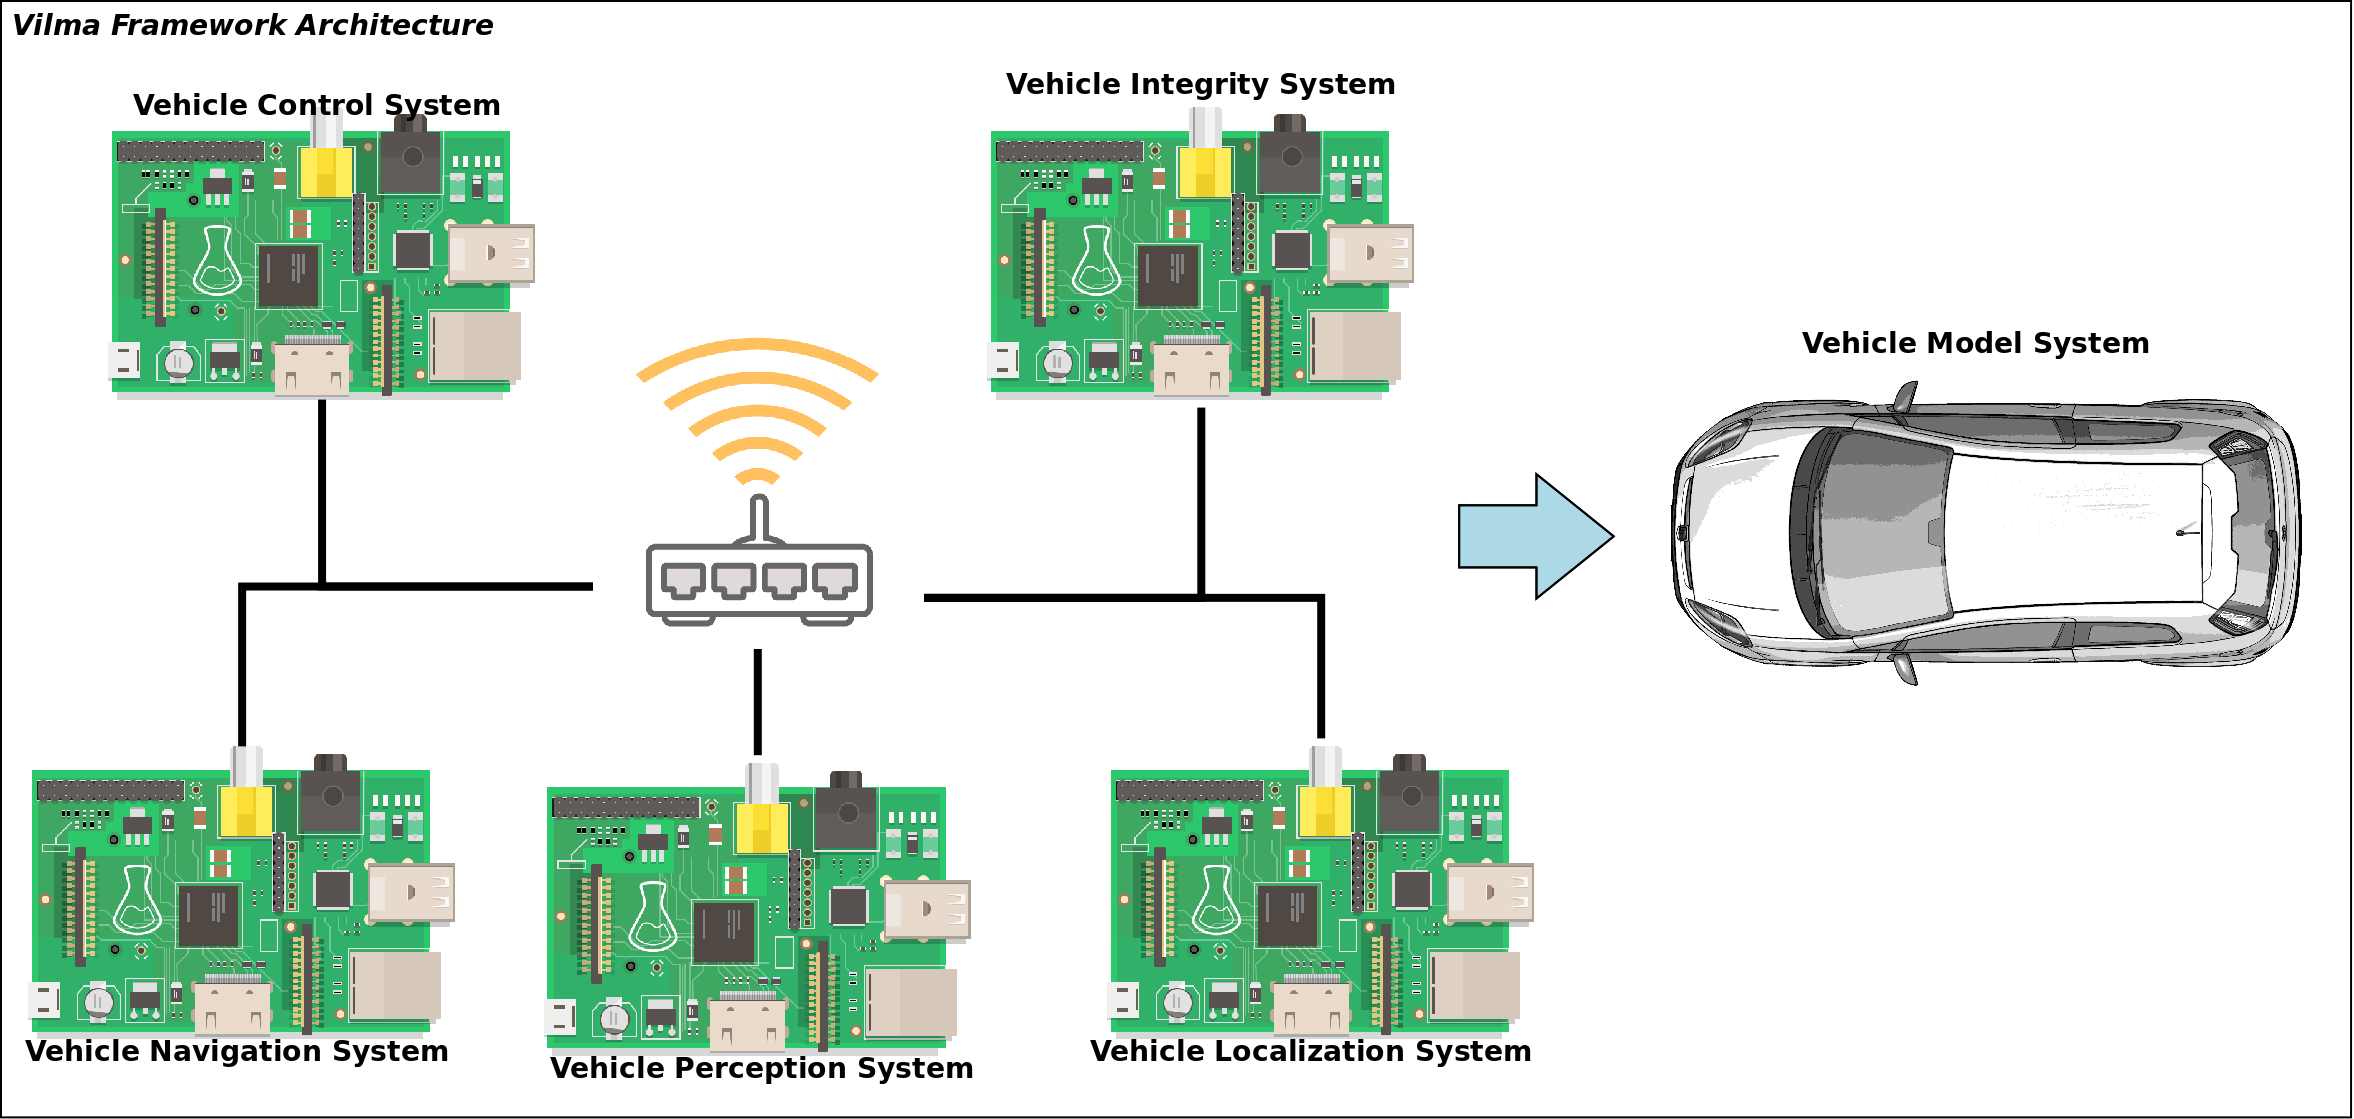
\includegraphics[width=200px,keepaspectratio]{imagens/VILMA_SYSTEM_ARCHITECTURE2}
%	\caption{Processamento descentralizado.}
%	\label{fig:VILMA_SYSTEM_ARCHITECTURE}
%\end{figure}

Tendo como principal objetivo deste estudo, o desenvolvimento de um sistema denominado "Vehicle Integrity System" (VIS), parte do projeto VILMA \cite{lma_vilma_website}, responsável por verificar e controlar os modos de operação do veículo, monitorar os estados dos outros módulos, supervisionar e coordenar os sistemas nos diferentes modos de operação, propor a tomada de decisões em caso de falhas dos componentes presentes na arquitetura do veículo, realizar o controle e registro de mensagens facilitando a manutenção e depuração do sistema durante a fase de desenvolvimento do projeto. Onde, para de atender o objetivo do trabalho, a arquitetura proposta deve garantir os seguintes requisitos:

\begin{itemize}
	\item propor uma arquitetura determinística com características para o desenvolvimento de sistemas críticos em tempo real;
	\item padronizar a interface de comunicação entre os sistemas presentes na arquitetura do veículo;
	\item fornecer uma interface que possibilite a integração de outros trabalhos ao sistema supervisório de forma ágil e baixa complexidade;
	\item oferecer um sistema supervisório que monitora o estado atual dos outros componentes do veículo;
	\item o sistema supervisório deve coletar informações sobre os demais componentes;
	\item o supervisor deve decidir se um componente está trabalhando de forma esperada ou não, e tomar decisões para solucionar problemas;
	\item as informações coletadas devem ser reportadas a interface de usuário do veiculo;
	\item além do controle comportamental e do gerenciamento operacional, o sistema supervisório deve monitorar a integridade dos demais componentes que implementem a interface fornecida pelo VIS;

%	\item to ensure a set of characteristics that the architecture of all the built robots will provide. For example, the real-time communication bandwidth guarantee for a n number of dispositives plugged into the robot;
	
	%\item to manage the interface between the real-time requirements of the manipulation tasks of the robot and the non-realtime computational intelligent process of the decision algorithms;
	
	%\item to standardize the communication interfaces among the robot dispositives and to standardize the communication interfaces among the main parts of the robot;
	
	%\item to develop an architecture capable of integrating and validating new technologies, such as different kinds of actuators and sensors;
\end{itemize}


% -------------------- NEW SECTION -------------------- 
% -------------------- NEW SECTION -------------------- 
% -------------------- NEW SECTION -------------------- 

\section{Proposed Architecture}\label{sec:proposed_architec}

Este trabalho propõe um sistema para o controle supervisório que utiliza o conceito convencional de modelagem por FSMs levando em consideração o problema de reconfiguração dinâmica para o veículo VILMA como uma potencial plataforma de desenvolvimento às outras pesquisas desenvolvidas no LMA \cite{lma_vilma_website}. São adotados os conceitos formais para a modelagem por FSM e DES para que o sistema supervisório realize à coordenação dos demais módulos, troca do modo de operação do veículo, monitoramento da integridade dos sistemas e gerenciamento dos estados de operação dos módulos. 

Tenha em mente que o controle supervisório, como o nome sugere, supervisiona apenas o que os demais sistemas estão informando a ele, para isso, é necessário que haja  uma interface comum entre os módulos presentes no veículo, onde em caso de mau funcionamento ou a ocorrência de um comportamento inesperado, o supervisor do veículo possa realizar a coordenação dos demais sistemas reagirem à situação em potencial. A plataforma abordada pode ser considerada como uma espécie co-piloto do VAT que diz ao veículo como suas atividades devem ser organizadas, que configuração utilizar em determinado momento, quando indicar falhas detectadas em algum sistema específico, etc.  

%
% operational_modes
\subsection{Operational Modes}\label{subsec:operational_modes}
O laboratório de mobilidade autônoma (LMA) desenvolve pesquisas para que o projeto VILMA possa executar tarefas para os modos de operação manual e autônomo. No modo de operação manual, o veículo é guiado por um operador humano de forma convencional. No modo de operação autônomo, o veículo é conduzido por um sistema de controle computacional que recebe dados de sensores, processa as informações coletadas e atua diretamente sobre seus atuadores mecânicos. Uma vez em modo autônomo, é esperado que o veículo execute tarefas sem que haja direta intervenção humana. A realização das operações autônomas são caracterizadas por um sub conjunto de modos operacionais, chamados de: \textit{Open Terrain}, \textit{Road Following}, \textit{Vehicle Following} e \textit{Teleoperation}.

\begin{itemize}
	\item \textit{Open Terrain}, o veículo opera em ambientes abertos, ou seja, qualquer tipo de terreno que possua vales, depressões, desertos, etc;
	\item \textit{Road Following}, o veículo move-se por uma estrada orientando-se por características presentes nesta via, por exemplo, placas, semáforos, etc.;
	\item \textit{Vehicle Following}, o veículo deve simplesmente seguir um outro carro a sua frente;
	\item \textit{Teleoperation}, o veículo deve executar tarefas comandadas remotamente;
\end{itemize}

A troca entre o modo de operação manual para o modo autônomo é feita diretamente pelo operador dentro do veículo. Uma vez que o automóvel encontra-se em modo autônomo, o condutor pode realizar a troca para o modo manual quando necessário ou assim que desejar.

Durante o desenvolvimento do projeto o veículo deve executar suas tarefas operando em modo de depuração, nesta fase é possível operar em modo autônomo sendo permitida a realização de testes dos componentes e módulos que sendo desenvolvidos, porém o controle manual deve estar sempre disponível ao operador, tendo prioridade superior a qualquer tarefa autônoma sendo executada. A depuração também deve contar com o sistema de registro e visualização das mensagens e o estado sobre a situação atual de cada módulo em execução. A Figura \ref{fig:VILMA_OPERATIONAL_MODE} ilustra os modos de operação e as possíveis trocas entre os modos.

\begin{figure}[h]
	\centering
	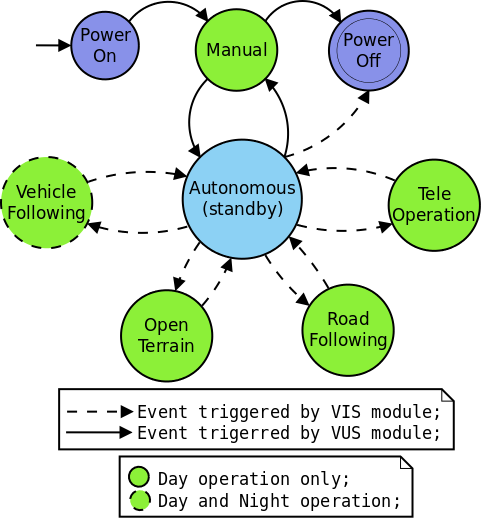
\includegraphics[width=200px,keepaspectratio]{imagens/VILMA_OPERATIONAL_MODE}
	\caption{Modos de operação do projeto VILMA.}
	\label{fig:VILMA_OPERATIONAL_MODE}
\end{figure}

O mecanismo de comutação entre modos operacionais é composto por um conjunto de funções que todos os módulos da arquitetura do veículo devem obedecer para que as tarefas sejam executadas sem comprometimento das atividades. Isso permite ao veículo ter o comportamento esperado, por exemplo, quando cada módulo estiver no estado \textit{Working}, então, estes módulos estarão prontos para executar funções específicas para cada um de seus sistemas. No entanto, pode haver o caso em que funções específicas a determinados modos de operação precisem ser combinadas para possibilitar que tarefas complexas sejam cumpridas de forma eficiente. Por exemplo, o módulo de navegação possui funções que realizam tarefas específicas nos modos de operação \textit{open errain} e \textit{road following}. A combinação dessas duas funções vai gerar uma nova funcionalidade, resultando em um novo comportamento durante seu deslocamento. Ainda tendo como exemplo o sistema de navegação, as informações captadas pelos sensores do módulo de localização e percepção (GPS, IMU, Bussola, Câmera, Laser Escâner, etc.) é que determinam quando deve ser feita a alteração entre os modos operacionais. 

Para exemplificar, considere a seguinte situação, suponha que o veículo esteja operando em modo \textit{open terrain}, e em algum momento o veículo recebe uma requisição do sistema de usuário para alterar seu destino. Neste momento, o sistema de usuário deve informar ao supervisório que houve uma requisição para alterar o destino da missão, consequentemente o supervisório direciona a informação para que o sistema de navegação instrua os sistemas de localização e posicionamento que continuem operando em modo \textit{open terrain}, caso a nova rota traçada possua uma estrada (detectada pelo tratamento das informações obtidas nos sensores), então os sistemas são informados que há uma estrada que leva ao destino e então devem alterar modo de operação adequado à aquela situação, no caso, \textit{road following}.

Sendo assim, podemos dizer que o veículo possui um sistema "inteligente" capaz de fornecer um conjunto abrangente de funções através da conjunção de funcionalidades, onde esta inteligência pode ser modelada por maquinas de estados para possibilitar o comportamento esperado pelo sistema supervisório, como no exemplo apresentado pela Figura \ref{fig:VILMA_OPERATIONAL_MODE_BEHAVIOR}.

\begin{figure}[h]
	\centering
	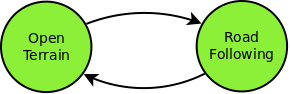
\includegraphics[width=200px,keepaspectratio]{imagens/VILMA_OPERATIONAL_MODE_BEHAVIOR}
	\caption{Comportamento de comutaçao FSM dos modos de operaçao.}
	\label{fig:VILMA_OPERATIONAL_MODE_BEHAVIOR}
\end{figure}

%
% modules_components
\subsection{Modules and Components}\label{subsec:modules_components}
O desenvolvimento de sistemas com arquitetura modular tem como objetivo melhorar a qualidade de software, reduzir o tempo necessário para integração de novas funcionalidades e agilizar a entrega dos trabalhos. Por este motivo, inicialmente o veículo VILMA é composto por sete sistemas, também chamados de módulos. Cada sistema e formado por componentes que realizam tarefas específicas. Os módulos e alguns dos principais componentes presentes na arquitetura do veículo podem ser vistos na Figura \ref{fig:VILMA_MODULES_COMPONENTS}.

\begin{figure}[h]
	\centering
	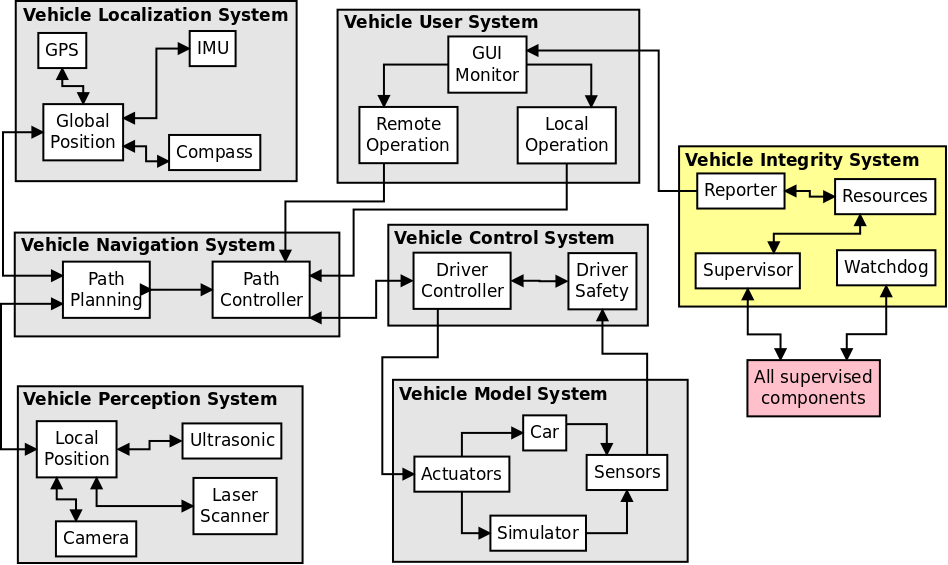
\includegraphics[width=270px,keepaspectratio]{imagens/VILMA_MODULES_COMPONENTS}
	\caption{Módulos e componentes do projeto VILMA.}
	\label{fig:VILMA_MODULES_COMPONENTS}
\end{figure}

A lista à seguir apresenta uma visão geral sobre os módulos e suas principais funções para o projeto VILMA.

\begin{itemize}
	\item \textit{Vehicle Model System} (VMS): é o sistema que representa o veículo, real e simulado, implementa a interface entre os atuadores e sensores de baixo nível presentes na arquitetura do veículo autônomo, onde são recebidos os comandos do VCS para a atuação e os sinais dos sensores são enviados ao próprio VCS;
	
	\item \textit{Vehicle Control System} (VCS): módulo responsável por controlar a atuação do veículo e garantir a segurança dos agentes envolvidos no ambiente de operação. Sua principal função é fornecer comandos para o controle de velocidade, aceleração e direção do veículo. O VCS gera sinais de baixo nível que acionam o sistema eletromecânico, informando a velocidade desejada, a aceleração necessária e a angulação da direção. Além disso o VCS, possui um \textit{feedback} cíclico de comunicação com o VNS para garantir que a velocidade e os comandos de direção estão sendo executados corretamente, levando em conta fatores ambientais, como a derrapagem das rodas entre outros;
	
	\item \textit{Vehicle User System} (VUS): o módulo VUS possibilita a interação do condutor ao automóvel, tanto em modo local quanto em modo remoto, possibilitado pela da utilização de câmeras instaladas no veículo para simular a visão do condutor. O operador controla a movimentação do automóvel através de um controle. Além disso o sistema deve fornecer uma interface gráfica possibilitando que o condutor saiba o estado do veículo em tempo real, bem como alertas e diagnósticos para a depuração durante o período de desenvolvimento;  
	
	\item \textit{Vehicle Perception System} (VPS): o sistema VPS utiliza diversos instrumentos, tais como, lasers escâneres, câmeras, sensores ultrassônicos para construir mapas digitais do ambiente em torno do veículo, ou seja, fornece o posicionamento local do automóvel. Os sensores toram o veículo capaz de reconhecer características do ambiente, por exemplo, estradas, áreas transitáveis, símbolos, etc. Também fornece o mapa digital para que o VNS possa realizar o planejamento da trajetória e a geração dos comandos de movimentação ao VCS para que sejam cumpridas as tarefas solicitadas;
	
	\item \textit{Vehicle Localization System} (VLS): bem como o sistema VPS, o módulo VLS utiliza de diversos instrumentos como GPS, IMU, bussolas eletrônicas e demais sensores que possibilitem a geração de mapas digitais da sua localização em escala global, diferentemente do sistema VPS que tem foco na geração de mapas locais. Ele também fornece as informações do mapa gerado para que o VNS possa realizar o planejamento de trajetória e geração dos comandos de movimentação ao VCS a fim de cumprir as tarefas necessárias;
	
	\item \textit{Vehicle Navigation System} (VNS): é responsável pela geração de comandos para à navegação do veículo afim de realizar a tarefa determinada pelo operador. Além disso, ele deve ser capaz de realizar o planejamento da trajetória até a localização desejada, calcular a velocidade e sua direção gerando as informações necessárias para que o VCS execute as tarefas de forma segura. Também deve	monitorar a posição do veículo bem como a execução das manobras a serem realizadas até seu destino;
	
	\item \textit{Vehicle Integrity System} (VIS): O módulo VIS é responsável por garantir a integridade do sistema que opera o veículo enquanto estiver em funcionamento. Sua principal função é monitorar e coordenar as atividades dos módulos para se obter o comportamento esperado do veículo. O controle destas atividades é realizado por meio de uma interface comum modelada por autômatos, que é gerenciada pelo componente \textit{Supervisor} responsável por determinar o comportamento das transições dos estados básicos de operação dos sistemas, como \textit{Standby}, \textit{Ready}, \textit{Working}, \textit{Internal Error}, etc. O VIS também realiza o roteamento dos dados entre os demais módulos, registra e publica as informações contento o status dos sistemas. Resumindo, o VIS atua como um co-piloto digital. Uma descrição mais aprofundada do sistema supervisório será apresentada no decorrer deste trabalho;
\end{itemize}
%
% states_transitions
\subsection{States and Transitions for Supervisory Control}\label{subsec:states_transitions}

Para que haja adequada coordenação das atividades executadas pelos sistemas presentes na arquitetura do veículo, é necessário que os componentes possuam um comportamento uniforme em relação ao VIS. Sendo assim, cada componente precisa implementar uma interface comum, também modelada por um conjunto de estados e transições que são reconhecidos pelo sistema de supervisão, possibilitando o gerenciamento das atividades sendo executadas, realizar o roteamento das mensagens necessárias à depuração e o armazenamento dos dados, etc. A coordenação entre módulos é responsável por determinar a sequencia das atividades e as condições que um sistema deve atender para que ele possa executar suas especialidades.

Sob a perspectiva do controle supervisório, os estados presentes neste sistema são: \textit{PowerOn}, \textit{PowerOff}, \textit{Standby}, \textit{Ready}, \textit{Working}, \textit{InternalError}, \textit{Emergency}, e \textit{Shutdown}.
Cada componente deve conter obrigatoriamente esses estados. Para um dado componente, o significado dos estado e o comportamento geral do veículo pode ser resumido da seguinte maneira.

\begin{itemize}

	\item em \textit{PowerOn} o condutor dá partida no veículo, neste instante o motor é iniciado porém o automóvel permanece estacionado aguardando as instruções do usuario sobre o modo de operação do veiculo;
		
	\item em \textit{Standby} o componente passa a estar inicializado e o veículo continua parado. Nesse estado, o sistema não está vinculado a um modo autônomo de operação, onde permanece aguardo as instruções do sistema supervisório sobre o modo de operação ou à instrução para que retorne ao modo manual;
	
	\item em \textit{Ready}, o componente está vinculado a um modo autônomo de operação mas ainda não está operado nesse modo, o veículo continua estacionado com o moto em funcionamento. O motivo pela separação entre os estados \textit{Standby e Ready} deve-se ao fato deste trabalho se concentrar no comportamento geral do veículo, onde existe a necessidade de uma clara separação temporal entre os estados onde o veículo possa retornar ao modo de operação manual e o estado onde ele esteja preparado para operar em modo autônomo. A separação temporal dos estados é necessária para à sincronização das atividades dos componentes antes que eles entrem no estado \textit{Working};
	
	\item uma vez em \textit{Working}, o componente está operando em um modo de operação autônomo e o veículo está em movimento. É neste estado que o algoritmo especifico do componente começa a ser executado para produzir seu comportamento esperado, por exemplo, a fusão sensorial do módulo VLS que integra os dados dos componentes GPS, IMU e bussola para produzir um mapa digital em escala global;
	
	\item em \textit{InternalError} e \textit{Emergency} o componente executa tarefas relevantes a manipulação de exceções geradas por seu algoritmo funcional ou respostas de emergência que comprometam o funcionamento geral do veículo;
	
	\item em \textit{Shutdown}, o componente executa um conjunto predefinido de rotinas preparando o veículo para ser desligado, retornando o sistema ao estado \textit{PowerOff};
	
	\item por fim, em \textit{PowerOff}, o sistema está desligado e nenhum sinal elétrico é fornecido ao componente;
\end{itemize}

As transições entre os estados consistem um conjunto de atividades que levam os componentes de um estado a outro. Para uma transição ocorrer ela deve ser disparada por um evento. Uma vez invocado, as atividades associadas a transição devem ser realizadas com sucesso para que o componente entre em um novo estado. O diagrama dos estados e as transições comuns ao sistema supervisório pode ser visto na Figura \ref{fig:VILMA_STATE_MACHINE2}. As especificações que representam restrições das atividades de cada módulo também podem ser moladas por uma autômatos para produzir um modelo de especificações composto. Em seguida, baseando-se na teoria de controle para eventos discretos (DES) podemos obter um modelo formal para o controle supervisório, como apresentado em \cite{event_systems}.

As especificações resultantes, descritas por uma FSM, formam uma cadeia contendo todas as atividades e sequências de transições permitidas para garantir que todas as especificações sejam atendidas, ou seja, quando algum dos módulos precisa realizar uma transição entre os estados da FSM que descrevem seu comportamento. Por exemplo, para entrar no estado \textit{Working} ou deixar o estado \textit{Working} e ir para o estado \textit{Standby} ou quando um módulo estiver realizando o tratamento de alguma exceção em \textit{InternalError}, todas as transições dos estados relacionados devem verificar suas restrições e obter a permissão do modulo supervisório antes que a transição ocorra. 

\begin{figure}[h]
	\centering
	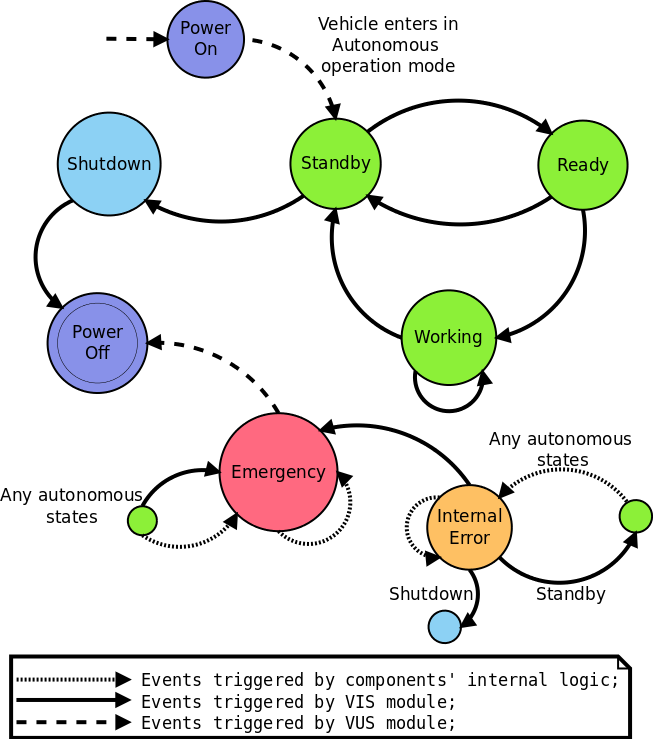
\includegraphics[width=250px,keepaspectratio]{imagens/VILMA_STATE_MACHINE2}
	\caption{Estados e transições dos componentes.}
	\label{fig:VILMA_STATE_MACHINE2}
\end{figure}

Embora cada componente contenha o conjunto de estados e transições obrigatórios, a questão sobre as atividades envolvidas nos estados e transições é transparente para o VIS. Em outras palavras, o VIS não conhece internamente a complexidade das tarefas executadas dentro dos estados ou durante as transições de um componente e não existe restrição que ele possua apenas estes estados e transições. As atividades envolvidas nas transições de cada componente podem ser diferentes daquelas presentes em outros componentes.

%
% formal_synthesis
\subsection{Approach of DES on Formal Synthesis }\label{subsec:formal_synthesis}

Após o modelamento que determina o comportamento dos módulos em termos de estados e transições, é possível formalizar a lógica do projeto VIS através de técnicas formais mais avançadas. 
Uma das possíveis metodologias é a teoria de controle para sistemas supervisórios de evento discreto \cite{event_systems}. 
A aplicação desta técnica exige que os estados e transições dos módulos sejam expressos em conjuntos de autômatos (chamados de modelos), enquanto o comportamento desejado do veículo seja expresso por outro conjuntos de autômatos (chamados especificações). 
Por exemplo, o comportamento de um módulo, seguindo as especificações do VIS como ilustrado na Figura \ref{fig:VILMA_STATE_MACHINE2}, pode ser representado por um automato $G = (Q,\Sigma,\delta,q_{0},Q_{m},q_{m-1})$, onde $Q$ é um conjunto de estados, exemplo, $Q =$ \{\textit{PowerOn, PowerOff, Standby, Ready, Working, InternalError, Emergency, Shutdown}\}, $\Sigma$ é um conjunto de transições, exemplo, $\Sigma =$ \{\textit{1,2,3,4,5,6,7,A,B,C,D,E,F,G,H,I,J,K,L,$\alpha$,$\beta$,...}\}, $\delta$ é a função de transição que especifica o novo estado após a transição do estado atual, como apresentado pela Tabela \ref{tab:func_transicao}, $q_{0}$ é o estado inicial, $q_{m-1}$ o estado final do componente e $Q_{m}$ é o conjunto de estados que indicam a conclusão de determinadas transições.

% Please add the following required packages to your document preamble:
% \usepackage{multirow}
\begin{table}[h]
	\centering
	\adjustbox{max height=\dimexpr\textheight-5.5cm\relax, max width=\textwidth}{
		\renewcommand{\arraystretch}{1.25}
		\begin{tabular}{|c|c|c|}
			\hline
			\multicolumn{3}{|c|}{$\delta(old state, transition) = new state$} \\ \hline
			Old state & transition & new state \\ \hline
			power-on & A & standby \\ \hline
			\multirow{4}{*}{standby} & B & ready \\ \cline{2-3} 
			& C & shutdown \\ \cline{2-3} 
			& D & internal error \\ \cline{2-3} 
			& E & emergency \\ \hline
			\multirow{4}{*}{ready} & F & working \\ \cline{2-3} 
			& G & standby \\ \cline{2-3} 
			& H & internal error \\ \cline{2-3} 
			& I & emergency \\ \hline
			\multirow{4}{*}{working} & J & standby \\ \cline{2-3} 
			& K & working \\ \cline{2-3} 
			& L & internal error \\ \cline{2-3} 
			& M & emergency \\ \hline
			\multirow{3}{*}{internal error} & N & standby \\ \cline{2-3} 
			& O & shutdown \\ \cline{2-3} 
			& P & internal error \\ \hline
			\multirow{2}{*}{emergency} & Q & power-off \\ \cline{2-3} 
			& R & emergency \\ \hline 
			shutdown & T & power-off \\ \hline
		\end{tabular}
		\renewcommand{\arraystretch}{1}
	}
	\caption{Exemplo da função de transição $\delta$ do modelo baseado na Figura \ref{fig:VILMA_STATE_MACHINE2}.}
	\label{tab:func_transicao}
\end{table}

Uma vez que cada módulo do sistema é modelado por um automato $G_{i}$, um modelo composto sobre o comportamento geral do veículo pode ser construído utilizando o procedimento chamado \textit{"synchronous product"}, representado pelo símbolo $\lVert$ \cite{event_systems_ebook}. O resultado do produto síncrono sobre todo $G_{i}$ é um novo automato que representa o comportamento "livre" (não controlado) das atividades simultâneas dos módulos. Ou seja, $G = G_{1} \lVert G_{2} \lVert G_{3} \lVert ... \lVert G_{n}$.  

Então, o comportamento determinístico do veículo pode ser imposto ao comportamento "livre" para se obter as estratégias para o controle supervisório esperados pelo VIS. Formalmente, tal comportamento também é expresso em autômatos, chamados autômatos de especificações. 
Ao impor as especificações do modelo composto de todos os componentes do veículo, um conjunto sequencial de transições pode ser obtido para serem executadas pelo VIS, garantindo que o comportamento do veículo atenda as especificações de controle. 

Ao utilizar esta abordagem, é possível sintetizar as estratégias de controle supervisório permitindo que o veículo possa lidar com situações distintas. Por exemplo, suponha que devido restrições de sincronização temporal, o VCS só possa entrar no estado \textit{Working} após o VNS estiver no estado \textit{Working}. Isso pode ser considerado como um dos requisitos que constituem o comportamento desejado para a inicialização de uma tarefa. Esse requisito pode ser expresso como uma especificação $S_{i}$, como apresentado na Figura \ref{fig:VILMA_TRANSITION_EXAMPLE}, onde os laços cíclicos representam outras possíveis transições que podem ocorrer no sistema.

\begin{figure}[h]
	\centering
	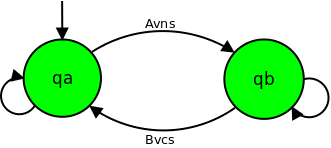
\includegraphics[width=200px,keepaspectratio]{imagens/VILMA_TRANSITION_EXAMPLE}
	\caption{Exemplo de uma especificação, $A_{vns}$: Transição do estado \textit{Ready} para \textit{Working} no módulo \textit{Vehicle Navigation System}, $B_{vcs}$: Transição do estado \textit{Ready} para \textit{Working} no módulo \textit{Vehicle Control System}.}
	\label{fig:VILMA_TRANSITION_EXAMPLE}
\end{figure}

O controle supervisório que garanta o comportamento dos módulos, como um todo, e que satisfaça a especificação imposta por $S_{i}$ pode ser obtido, dentre outras formas, pelo algoritmo chamado \textit{SUPCON} \cite{supcom_wonham1987supremal}. Sua função é gerar sequencias de eventos sob a forma de outro automato $V$, exemplo, $ V = SUPCON(G,S_{i})$, que pode ser implementado para garantir o comportamento determinístico de todo o sistema do veículo.

Ao expressar todos os requisitos sobre o comportamento do veículo em autômatos de especificações, torna-se possível desenvolver um método de controle sofisticado, que quando implementado pelo VIS garantirá que veículo atenda a todos os requisitos impostos pelos demais módulos. Essa abordagem formal permite o desenvolvimento sistemático e correto para as estratégias de controle supervisório, além de permitir a introdução da "inteligencia artificial programada" para o comportamento geral do veículo, e consequentemente obter um auto grau de autonomia.

% DOWNLOAD SOFTWARE DES http://www.control.utoronto.ca/~wonham/wonham.html

% -------------------- NEW SECTION -------------------- 
% -------------------- NEW SECTION -------------------- 
% -------------------- NEW SECTION -------------------- 
\section{Architecture Components}\label{sec:architec_components}

O desenvolvimento de software para veículos autônomos terrestres é uma tarefa complexa. Não se trata apenas em escrever códigos que implementem algoritmos específicos para que o automóvel faça isso ou aquilo. O processo de desenvolvimento inclui implementar, integrar, simular, testar, etc. todos os componentes de software necessários para tornar o sistema uma plataforma funcionalmente viável. Para isso, muitos aspectos devem ser considerados pois situações adversas geralmente costumam ter diferentes requisitos e objetivos, não existe um manual passo-a-passo que diz corretamente como tudo deve ser feito. Porém, veículos autônomos apresentam uma característica em comum, este tipo de aplicação normalmente precisa atender requisitos temporais rigidamente estabelecidos, onde as tarefas precisam ser executadas dentro dos prazos determinados ou falhas catastróficas poderão ocorrer, causando o mal funcionamento do sistema e podendo levar danos com vítimas fatais.

Para atender aos aspectos descritos normalmente é necessário que a aplicação seja desenvolvida em uma plataforma que possua um sofisticado ambiente de hardware e software para garantir os critérios determinísticos de um sistema crítico de tempo real. Porém, este trabalho concentra seus esforços em prover uma arquitetura com foco em tecnologias e metodologias baseadas puramente em software, capazes de realizar tarefas críticas em tempo real, reduzindo o custo e tempo para a prototipagem do projeto VILMA.

%Antes de descrever as especificações do sistema de controle supervisório, será apresentado brevemente conceitos para elucidar a compreensão do ambiente proposto, visando atender os requisitos necessários para a realização deste projeto. Vale ressaltar que a metodologia de escolha para a proposta da arquitetura a ser desenvolvida baseia-se nos estudos e resultados previamente realizados por outros pesquisadores, não sendo considerada uma escolha definitiva.

A Figura \ref{fig:VILMA_ENV_OVERVIEW_NET} apresenta o esquema dos principais elementos que compõem ambiente de desenvolvimento proposto para o projeto VILMA.

\begin{figure}[h]
	\centering
	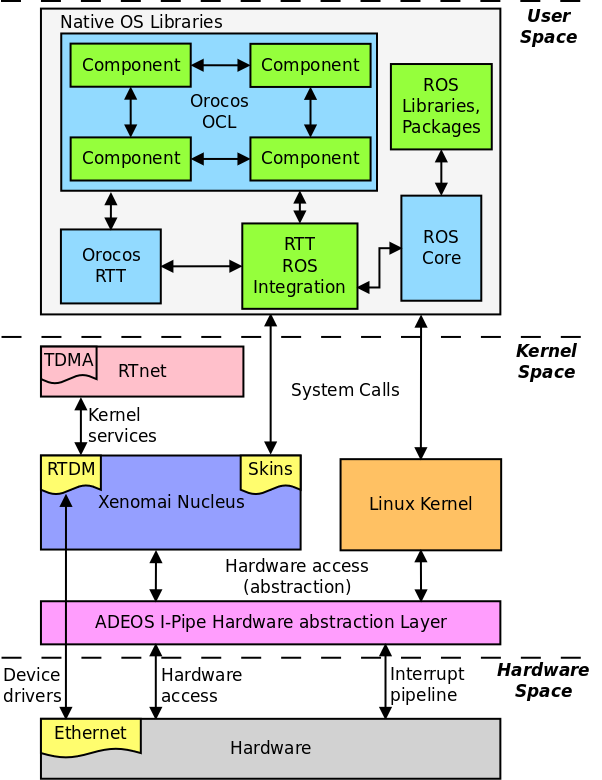
\includegraphics[width=250px,keepaspectratio]{imagens/VILMA_ENV_OVERVIEW_NET.png}
	\caption{VILMA platform, infraestrutura dos componentes utilizados para o desenvolvimento do projeto VILMA.}
	\label{fig:VILMA_ENV_OVERVIEW_NET}
\end{figure}

%
% linux
\subsection{Linux}\label{subsec:linux}

Linux is, in simplest terms, an operating system. It is the software on a computer that enables applications and the computer operator to access the devices on the computer to perform desired functions. The operating system (OS) relays instructions from an application to, for instance, the computer's processor. The processor performs the instructed task, then sends the results back to the application via the operating system \cite{linux_barabanov1997}.

One of the most noted properties of Linux is where it can be used. Windows and OS X are predominantly found on personal computing devices such as desktop and laptop computers. Other operating systems, such as Symbian, are found on small devices such as phones and PDAs, while mainframes and supercomputers found in major academic and corporate labs use specialized operating systems such as AS/400 and the Cray OS.

Linux, which began its existence as a server OS and Has become useful as a desktop OS, can also be used on all of these devices. “From wristwatches to supercomputers”, is the popular description of Linux' capabilities. \cite{linux_foundation}

%
% xenomai
\subsection{Xenomai}\label{subsec:xenomai}

Xenomai \cite{xenomai_api} is a real-time development framework cooperating with the Linux kernel, in order to provide a pervasive, interface-agnostic, hard real-time support to user-space applications, seamlessly integrated into the GNU/Linux environment \cite{xenomai_x_linux}. The Xenomai drivers has the RTDM (Real-Time Driver Model) which composes the following modules: CAN Devices, Real-time IPC Devices, Serial Devices, and Testing Devices \cite{rtdm_Kiszka}.

%
% rtnet
\subsection{RTnet}\label{subsec:rtnet}

With Ethernet, the communications are not deterministic because of the collision which can occur between several host on a network with a hub, or because of the unknown latency in the case of the switch. The deterministic communication is not allowed by the Ethernet protocol because of the possibility of collisions which can occurs and supported by the mechanism CSMA/CD (Carrier Sense Multiple Access/Collision Detection) \cite{rtnet_IEEE_so53551}.

RTnet is a protocol stack which run between the Ethernet layer and the application layer (or IP layer) with hard real-time requirements \cite{rtnet_org}. It aims, through the use of time intervals (time-slots), is to make deterministic communication, by disabling the collision detection CSMA/CD, and prevent buffering packet in the network. RTnet is a software developed to run on Linux kernel with RTAI or Xenomai real-time extension. It exploits the real time kernel extension to ensure the determinism on the communication stack. In this aim, all the instructions related to this protocol makes use real time kernel functions rather than those of Linux, which bound latencies to the execution times and latencies of interruptions which provide deterministic’s communication \cite{rtnet_from_xenomai}.

The protocol supports both real-time and non-real-time communication. Applications are able to reserve a portion of the available bandwidth to transmit real-time data, organised in streams and requires a fully-connected communication medium, such as a common bus, Ethernet, or a radio medium, where every message sent can be received directly by all other nodes. Broadcast capabilities are needed to enable automatic addition and removal of nodes and to synchronize the nodes' clocks.\cite{rtnet_1559870}. 
At the same time the network uses the remaining bandwidth for best-effort traffic. The network is scheduled dynamically, using standard real-time scheduling algorithms normally used to schedule tasks on a CPU.
Nodes and streams may be flexibly added and removed. The protocol can be used in any local area environment where a distributed protocol is appropriate and where Quality of Service (QoS) support and flexibility is required \cite{rtnet_Wulf03acompact}.

%
% ros
\subsection{ROS}\label{subsec:ros}
The robot software is base on the ROS (Robot Operating System) \cite{ros_components}, an meta-operating system for robots. It provides the services like hardware abstraction, low-level device control, and message-passing between processes.
ROS is composed by the operating system commands that manage the packages, and a suite of user contributed packages (organized into sets called stacks) that implement functionality such as simultaneous localization and mapping, planning, perception, simulation etc \cite{ros_gentle_introduction} \cite{ros_bmw_sticha}.

%
% orocos
\subsection{OROCOS}\label{subsec:orocos}
Orocos \cite{orocos_Project_IEEE} is the acronym of the Open Robot Control Software project. The project's aim is to develop a general purpose, free software, and modular framework for robot and machine control. The Orocos project supports 4 C++ libraries \cite{orocos_manual}: the Real-Time Toolkit, the Kinematics and Dynamics Library, the Bayesian Filtering Library and the Orocos Component Library.
The Orocos Real-Time Toolkit (RTT) is not an application in itself, but it provides the infrastructure and the functionalities to build robotics applications in C++.
The emphasis is on real-time, on-line interactive and component based applications \cite{orocos_Cobem}.

A integração entre OROCOS e ROS pode ser realizada utilizando a biblioteca \textit{rtt\_ros\_integration} \cite{rtt_ros_integration}. Uma breve descrição sobre como essa integração acontece é apresentada a seguir:

\begin{itemize}
	\item \textbf{Data flow} Os componentes de OROCOS possuem estruturas chamadas de \textit{data ports}, meio por onde os componentes trocam dados entre si e os processos. No sistema ROS esse mecanismo é equivalente aos \textit{nodes} , que realizam a troca de informações entre os \textit{topics}. Através da biblioteca de integração, componentes OROCOS podem publicar dados para os \textit{topics} do ROS e vice versão;
	
	\item \textbf{Properties} Componentes OROCOS também possuem variáveis chamadas \textit{property}, ao passo que \textit{nodes} em ROS possuem os chamados \textit{parameters}. Assim, a biblioteca torna possível que os componentes OROCOS leiam os parâmetros oriundos dos \textit{server parameter} em ROS;
	
	\item \textbf{Deployment} O desenvolvimento dos componentes em OROCOS são executados em combinação com os \textit{nodes} em ROS através da utilização de somente um único \textit{script} de inicialização (chamado de \textit{launch});
	
	\item \textbf{Generation and Building} Ambos ROS e OROCOS possuem macros e \textit{scripts} disponíveis para a geração dos componentes em OROCOS e os pacotes ROS através do meta-compilador Catkin \cite{catkin_ros} \cite{catkin_gentle_intro};
\end{itemize}

Em resumo, o \textit{framework} ROS é utilizado para criar uma interface de comunicação entre os componentes e o sistema OROCOS realiza o encapsulamento da API do \textit{kernel} de tempo real Xenomai possibilitando a definição e execução de tarefas em tempo real ou não.

% -------------------- NEW SECTION -------------------- 
% -------------------- NEW SECTION -------------------- 
% -------------------- NEW SECTION -------------------- 
\section{Implementation}\label{sec:implementation}

O sistema de controle supervisório realiza o gerenciamento e a coleta de informações dos outros componentes do veículo por meio de uma interface comum que precisa ser implementada por cada um deles. Assim, deve-se fornecer aos demais pesquisadores do LMA meios para que possam integrar seus projetos ao sistema supervisório possibilitando a gerenciamento de seus sistemas de forma "transparente". Além disso, após a integração o consumo de recursos do sistema precisa ser o mínimo possível para não impactar na performance funcional dos projetos. 

O supervisório deve também garantir a integridade dos componentes necessários para à execução das tarefas durante a navegação autônoma, para isso, uma mensagem será solicitada periodicamente a cada componente presentes no sistema, com o a finalidade de garantir a presença e seu adequado funcionamento. Por fim, é necessário repassar as informações coletadas de cada sistema para um componente de interface com usuário. O objetivo é que o operador possa dizer se um componente está se comportando corretamente ou não, sem ter qualquer conhecimento do supervisor.

%
% module_behavior
\subsection{A General Description of Module Behavior}\label{subsec:module_behavior}

Uma vez solicitado pelo operador para que o veículo atue no modo de operação autônomo, o VIS deve solicitar à todos os componentes gerenciados realizem seu procedimento interno de inicialização, isso pode incluir a verificação de sensores, testar os atuadores, checar a presença de outro componente na rede, etc.
Então, caso nenhum dos componentes detecte falhas durante sua inicialização, eles devem informar ao sistema supervisório que estão inicializados e prontos para operar em modo de operação autônomo, assim o VIS solicita a todos os componentes a transição para o estado \textit{Standby} e permaneçam aguardando novas instruções. 

Uma vez em \textit{Standby}, o VIS pode instruir os componentes para o estado \textit{Shutdown}, em caso de falhas detectadas por algum componente, ou se prepararem para um modo de operação específico. Os componentes poderão mover-se para o estado \textit{Ready} caso tenham realizado seus processos configuração que garantam sua ativação ao modo de operação especificado, conforme instruções do VIS.  Assim que o processo seja cumprido, o VIS pode instruir aos componentes que comecem a operar, levando-os ao estado \textit{Working}. Estando neste em \textit{Working}, o VIS pode instruir que os componentes retornem ao estado \textit{Standby}, caso seja necessária a troca do modo de operação específico.

Erros operacionais, representados pelo estado \textit{InternalError}, podem ocorre quando um componente está em qualquer dos seguintes estados: \textit{Standby}, \textit{Ready} e \textit{Working}. Cabe exclusivamente ao componente decidir o que constitui uma erro interno. Quando um exceção ocorrer, o VIS pode instruir ao componente em questão tanto para que este realize o procedimento de reinicialização ou seu desligamento. Caso seja reiniciado, o componente poderá retornar ao estado \textit{Standby}.

Emergências, representadas pelo estado \textit{Exception}, podem ocorrer quando um componente está em algum dos seguintes estados: \textit{Standby}, \textit{Ready}, \textit{Working} ou \textit{InternalError}. O supervisório trata a uma emergência por duas formas, de acordo com a gravidade do ocorrido ou por meio da decisão do operador, que pode instruir o componente a ser reiniciado e retorná-lo ao estado \textit{Standby} após a emergência ser solucionada, ou optar pelo desligamento do sistema.

A estrutura de estados e transições apresentada pela Figura \ref{fig:VILMA_STATE_MACHINE2} deve ser implementada pelo VIS e por cada componente como um processo de software baseado em eventos (\textit{event-driven}).  VIS interage com os outros componentes com base nesta estrutura para realizar a supervisão das atividades do veículo. Estes estados e transições definem o comportamento dos componentes gerenciados pelo VIS. Entretanto, não existe nenhuma restrição para que os componentes possuam estados e transições próprias. Um componente pode possuir quantos estados e transições forem necessárias a suas atividades específicas, a única diferença é que estes não serão reconhecidos pelo VIS. 

Para exemplificar, considere o componente responsável pela navegação do automóvel (\textit{Planning}). O estado \textit{Working} do componente \textit{Planning} pode ser dividido em um sub-conjunto contendo sub-estados, por exemplo, \textit{Working-open-terrain}, \textit{Working-teleoperation}, etc., estes sub-estados certamente vão possuir diferentes conjuntos de tarefas. Em particular, no sub-estado \textit{Working-teleoperation}, o componente \textit{Planning} pode não possuir tarefas específicas, ou seja, uma transição "vazia". No entanto, quando o VIS requisitar que todos os componentes realizem a transição para o estado \textit{Working} com o veículo operando em modo \textit{Teleoperation}, o componente \textit{Planning} move-se para esse estado, embora internamente esta transição possa ser indiferente quanto a transição realizada a partir do estado \textit{Standby}.

Ao adotar o diagrama de estados e transições apresentado pela Figura \ref{fig:VILMA_STATE_MACHINE2} como uma interface padrão de comportamento entre o VIS e os demais componentes do projeto VILMA, suas atividades internas tornam-se transparentes para o sistema de supervisão, garantindo gerenciamento das atividades sem que o VIS precise interferir na estrutura e operações individuais de cada componente.

%
%
\subsection{VIS Software Processes}\label{subsec:vis_software_processes}

O módulo VIS é constituído por dois processos de software, um baseado em processo \textit{event-driven}, que possui a finalidade de proporcionar a coordenação das atividades entre os componentes sinalizando a troca de seus estados. E o outro baseado em processo periódico, \textit{periodic-tasks}, para monitoramento da integridade dos componentes presentes na arquitetura do projeto VILMA.

O processo \textit{event-driven} é responsável pela execução de quatro tarefas: 
\begin{enumerate}
	\item Gerenciar a sequência de alteração dos modos operacionais do veículo;
	\item Gerenciar a transição entre os estados de operação dos demais componentes;
	\item Realizar o roteamento dos dados entre os componentes;
	\item Coletar informações sobre o estado do veículo e seus componentes;
\end{enumerate}

Já o processo periódico é responsável por monitorar continuamente a integridade dos demais componentes durante todo o tempo em que o veículo estiver em funcionamento. A verificação dos demais componentes é realizada pelo recebimento uma mensagem \textit{time-stamped}, chamada de \textit{heartbeat}, em uma frequência predefinida. Se o período de chegada dos \textit{heartbeats} de um componente corresponder ao valor pré-definido, então, o módulo VIS assume que este componente em particular está funcionando normalmente.

Caso o VIS não receba o \textit{heartbeat} de um componente, então, o VIS assumirá que aquele componente em particular não está funcionando corretamente, assim, ele irá instruir todos os componentes a se moverem para o estado \textit{Standby}, para avaliação da possível falha. O processo periódico do VIS precisa enviar uma mensagem de \textit{heartbeat} ao VNS para que ele possa monitorar a integridade operacional do VIS, caso as mensagens de \textit{heartbeat} do VIS não cheguem ao VNS, então, deve instruir o sistema ao procedimento de emergência.

%To illustrate the applicability of the proposed supervisory control system, we consider a simple example with the scenario as shown in Figure 8. We assume that the vehicle is given a mission to reach some target through several waypoints sequentially. Upon receiving the mission to go to the target place, the mission planner depending on a satellite-based digital map will produce a task list that relates to a series ofwaypoints “w101, wl02, w103, ~104‘: which is a rough trajectory that the vehicle can traverse through, The task list and the related task specifications could be obtained accordingly, as shown in Table 1.

%Using the advanced functions “Goto” from the behavior library, the “AwlOl” task could be simply described as “Goto(SPEED, wlol)”, which means to go to the waypoint denoted by wlOl’s coordinate at a speed limited by the value indicated by “SPEED. Under the supervision of the module coordinator, the CIC will instruct all related modules to enter “Working” state and thcn call the parameterized “Goto” function. With the positioning and terrain information, the vehicle will automatically begin the “cross country” behavior and adjust to the suitable moving speed, which is the given max speed for it is traversing on plain. To save power and

%computational resource, only the necessary sensor, i.e. the UTVM’s stereovision device will he used. The CCD camera for road segment module (RSM) will be off at this moment. When the vehicle is within a given close distance to the waypoint “wlol”, the “AwlOl” task is completed. The execution of the next task is similar to the fmt one. When starting the task “AwlOY, the built-in behavior supervisor of “Goto” function will automatically switch to the “road following” behavior since a road is nearby. .Only RSM’s CCD will be used and the stereovision device will be tumed off temporarily. After completing task “AWIO~”, the vehicle will go back to “cross country” behavior for task “ A w l W . When entering the grassland terrain, the “cross country” function will automatically adjust the speed to a lower level

Para exemplificar este cenário, suponha que a frequência das mensagens de \textit{heartbeat} para todos componentes (exceto o VIS) seja configurara para $1Hz$. Essa seleção deve ser baseada considerando a distancia que o veículo percorrerá a partir do momento que a falha de um componente seja detectada pelo VIS até o instante em que o veículo estiver totalmente parado. Este deslocamento será chamado de distância de frenagem (\textit{fail-stop}).

Suponha que a velocidade é definida por \textit{s} em \textit{km/h} e a distância de parada do veículo por \textit{d} em metros. Com uma frequência de $1Hz$ para as mensagens de \textit{heartbeats}, o VIS conseguirá detectar uma falha em um componente a cada 1 segundo. Durante este tempo e em condições ideais, o veículo terá percorrido uma distancia de \textit{1000s/3600} metros até sua parada total. Assumindo que o tempo necessário para que o VIS instrua ao sistema responsável pelos atuadores que realize a parada do veículo seja desprezível, então a distancia \textit{fail-stop} será \textit{d + (1000s/3600)} metros. Ainda como exemplo, assumindo \textit{s = 10km/h}, \textit{d = 4m} e \textit{(1000s/3600) = 2.8m}. Assim a distancia \textit{fail-stop} quando o veículo estiver se movendo a velocidade de \textit{10km/h} será \textit{4+2.8 = 6.8} metros, em condições ideais.

% -------------------- NEW SECTION -------------------- 
% -------------------- NEW SECTION -------------------- 
% -------------------- NEW SECTION -------------------- 
\section{Conclusion}\label{sec:conclusion}



A discussão sobre o projeto do controle supervisório que estabeleça um comportamento determinístico para os demais sistemas do veículo autônomo ilustra como a robustez e segurança do projeto pode ser reforçada utilizando as metodologias apresentadas.

Neste sentido, foi apresentado o estudo e modelagem para o sistema de controle supervisório que compõe à arquitetura proposta para a plataforma de desenvolvimento do veículo VILMA e sua implementação preliminar a fim de atender seu objetivo determinado, realizar operações autônomas em ambiente terrestre de forma segura.

De acordo com esta arquitetura, o gerenciamento operacional do veículo é obtido através da adoção de uma interface uniforme modelada por FSM, que utiliza transições genéricas para a comutação dos estados referentes as tarefas executadas em cada componente no veículo. Esta estrutura representa um conjunto comportamental para os componentes gerenciados pelo VIS concebido com base nesta estrutura possibilitando que o sistema possua elevado grau de determinismo, ou seja, o veículo possui comportamento esperado durante a execução de suas tarefas.

Além disso, mostramos que esta arquitetura pode facilitar a implementação para estratégias de controle mais sofisticados através de técnicas formais, como no caso dos DES, onde o controle supervisório baseado na metodologia de eventos discretos podem elevar o grau de autonomia do veículo, e representa um próximo passo para o desenvolvimento do veículo autônomo inteligente VILMA.

Também foi proposto uma plataforma de desenvolvimento formada por um arcabouço tecnológico com foco no objetivo em tornar o trabalho do grupo de pesquisa do projeto VILMA padronizado, consolidando a agilidade, o baixo custo para o desenvolvimento do protótipo e sua continuidade uma vez que todas as ferramentas são bem documentadas e bastante difundidas. Essas tecnologias são amplamente utilizadas e consolidadas em equipamentos industrias e grupos de pesquisa. 

A integração entre os sistemas de baixo nível (Linux, Xenomai, Ethernet e RTnet), possibilita à obtenção de resultados dentro do escopo dos sistemas críticos de tempo real com processamento distribuído, garantindo os requisitos necessários para a viabilidade da aplicação.

A integração entre as estruturas em nível de usuário (ROS e OROCOS), reforça a ideia de agilidade e simplificação para o desenvolvimento das pesquisas desenvolvidas no LMA, inicialmente essa integração é baseada somente nas funcionalidades entre para o fluxos de dados entre os componentes dos \textit{frameworks} utilizados.		

Enquanto ROS possui bom suporte para a componentes distribuídos através da rede Ethernet, OROCOS oferece suporte à tarefas de comunicação entre componentes que necessitem de garantias temporais. Isso combina o melhor dos dois mundos: o controle em tempo real de baixo nível é tratado por um conjunto de componentes OROCOS-RTT que controla diretamente a troca de estados, gerencia os modos de operação adequados, verifica constante da integridade de cada sistema e ainda torna a comunicação entre os componentes visível para toda a rede dos sistemas ROS.

Por fim, a integração torna os componentes OROCOS como sendo componentes ROS, sem que haja quebra nos requisitos de tempo real entre os componentes OROCOS-RTT. Permitindo que sejam utilizadas as diversas ferramentas desenvolvidas para ROS, por exemplo, \textit{rviz} e \textit{rxplot}, para visualizar a comunicação entre os controladores.

% -------------------- NEW SECTION -------------------- 
% -------------------- NEW SECTION -------------------- 
% -------------------- NEW SECTION -------------------- 
% use section* for acknowledgment
\subsection*{Acknowledgment}\label{sec:acknowledgment}
The authors would like to thank...
% trigger a \newpage just before the given reference
% number - used to balance the columns on the last page
% adjust value as needed - may need to be readjusted if
% the document is modified later
%\IEEEtriggeratref{8}
% The "triggered" command can be changed if desired:
%\IEEEtriggercmd{\enlargethispage{-5in}}
% references section
% -------------------- NEW SECTION -------------------- 
% -------------------- NEW SECTION -------------------- 
% -------------------- NEW SECTION -------------------- 
\bibliographystyle{IEEEtran}
\bibliography{referencias}

% that's all folks
\end{document}